\chapter{Réalisations}\label{ch:realisations}

Après avoir exploré en détail la conception et la structure de l'API Pipeline documentaire, je me tourne maintenant vers sa réalisation concrète. Ce chapitre mettra en lumière la mise en œuvre pratique du projet, en alignant chaque étape avec les concepts élaborés précédemment. Des exemples de code viendront illustrer la manière dont les idées abstraites se traduisent en fonctionnalités fonctionnelles.

La réalisation de ce chapitre se décompose en deux sections principales. La première section se concentrera sur la démonstration des fonctionnalités clés du Pipeline documentaire. Plutôt que d'expliquer chaque aspect du projet en détail, ce segment mettra en avant les fonctionnalités principales de l'API. En utilisant des extraits de code pertinents, je suivrai l'évolution des composants essentiels, en mettant en évidence leur rôle dans l'importation et le traitement de fichiers.

La seconde section se focalisera sur une mission frontend spécifique qui illustre l'intégration pratique de l'API nouvellement créée. Plus précisément, j'explorerai comment la page d'importation des fichiers de transactions de carburant dans le projet Gestion de parc (Figure~\ref{fig:architecture}, page~\pageref{fig:architecture}) a été modifiée. Plutôt que d'utiliser l'ancienne API, cette page a été adaptée pour tirer parti de la puissance du nouveau Pipeline documentaire. Des exemples de code détaillés montreront comment ces modifications ont été apportées.

En réunissant la théorie et la pratique, ce chapitre offre un aperçu complet de la réalisation du projet, en montrant comment les concepts élaborés ont été traduits en un système fonctionnel.

\section{Pipeline Documentaire}\label{sec:pipeline-documentaire}

Cette première section plonge au cœur du projet Pipeline documentaire. Je commencerai par examiner le processus d'installation du projet dans un environnement de développement. Cela inclura la préparation de l'infrastructure nécessaire (conteneurs Docker) à l'exécution de l'API et la configuration de Laravel. De plus, je me pencherai sur les migrations de base de données indispensables pour assurer la cohérence des données et le bon fonctionnement de l'API. La section se poursuivra en explorant les modèles qui correspondent aux tables de la base de données.

Le cœur de cette section portera sur le processus clé de l'API : l'importation d'un fichier. Je décomposerai ce processus complexe en étapes gérables, en mettant en évidence les opérations importantes qui se produisent en arrière-plan lorsqu'un fichier est soumis à l'API. Des exemples de code accompagneront cette exploration, illustrant chaque étape du processus.

Enfin, j'aborderai l'aspect crucial des tests. La fiabilité et la robustesse de l'API sont essentielles pour assurer un fonctionnement sans faille.

En somme, cette première section plongera profondément dans l'API Pipeline documentaire, de sa mise en place à son fonctionnement concret. Chaque aspect exploré contribuera à la construction d'une base solide pour la section suivante, où j'examinerai l'intégration de l'API dans une mission frontend spécifique.

\subsection{Installation pour le développement}

Pour amorcer le développement de l'API, il est impératif de cloner deux projets à partir du dépôt GitLab de l'entreprise. Le premier de ces projets, intitulé \Verb|pipelinedoc-docker|, renferme un ensemble de fichiers essentiels. Ce dépôt inclut notamment un \Verb|Dockerfile| (\Verb|app.dockerfile|) ainsi qu'un fichier \Verb|docker-compose.yml|. Il abrite également une structure de dossiers (Figure~\ref{fig:pipelinedoc-docker-folders}) comprenant le fichier de configuration Nginx (\Verb|app.conf|), le répertoire destiné au code de l'API (\Verb|apps|) ainsi que d'autres dossiers de substitution nécessaires au projet.

\begin{wrapfigure}{l}{0.32\textwidth}
    \centering
    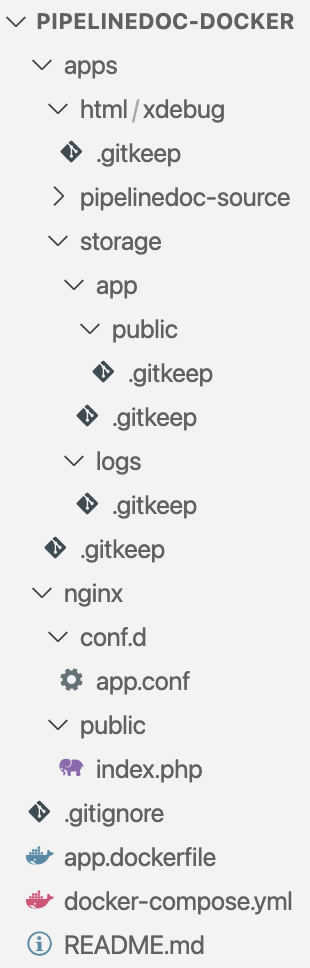
\includegraphics[width=0.30\textwidth]{img/pipelinedoc-docker-folders}
    \caption{La structure des dossiers du projet \Verb{pipelinedoc-docker}.}
    \label{fig:pipelinedoc-docker-folders}
\end{wrapfigure}

Le second projet, baptisé \Verb|pipelinedoc-source|, renferme le code source de l'API Pipeline documentaire. Ce dernier devra être cloné dans le dossier approprié au sein du projet \Verb|pipelinedoc-docker|. Cette étape est primordiale pour établir la connexion entre l'infrastructure Docker mise en place et le code de l'API à développer.

Les fichiers \Verb|app.dockerfile|, \Verb|docker-compose.yml| et le fichier de configuration Nginx sont essentiellement les mêmes que les fichiers présentés pour la production (Code source~\ref{code:dockerfile-prod}, page~\pageref{code:dockerfile-prod}; Code source~\ref{code:docker-compose-prod}, page~\pageref{code:docker-compose-prod}; Code source~\ref{code:nginx-conf-prod}, page~\pageref{code:nginx-conf-prod}). Cependant, bien qu'ils soient plus simples, ils ne contiennent pas toutes les instructions présentes dans ces fichiers.

Dès que les deux projets sont clonés, les conteneurs Docker peuvent être démarrés avec la commande suivante : \Verb|docker compose up|. Ensuite, le développeur doit créer le fichier \Verb|.env| pour le projet, contenant toutes les variables environnementales nécessaires, telles que les détails des connexions à la base de données, les URL et les jetons vers d'autres services, ainsi que d'autres paramètres de configuration. L'étape suivante consiste à installer les dépendances avec la commande \Verb|composer install| et à les mettre à jour avec la commande \Verb|composer update|. Ces commandes utilisent le fichier \Verb|composer.json| pour installer et mettre à jour les dépendances répertoriées avec leurs numéros de version. Ce projet inclut non seulement des dépendances publiques, mais également des dépendances développées et maintenues par l'entreprise dans son propre dépôt privé. Ces paquets privés sont ce que l'on appelle les \foreignquote{french}{cores}, comme nous l'avons mentionné précédemment (Figure~\ref{fig:architecture}, page~\pageref{fig:architecture}; Sous-section~\ref{subsec:cores}, page~\pageref{subsec:cores}).

Il reste encore trois petites étapes pour installer et démarrer complètement le projet : il faut lancer la commande \Verb|php artisan migrate:install|\footnote{Artisan est l'outil de ligne de commande intégré de Laravel, permettant d'effectuer diverses tâches liées au développement et à la gestion de projets Laravel.} pour créer la table \Verb|migrations| dans la base de données. Ensuite, il faut exécuter la commande \Verb|php artisan migrate| pour créer les tables nécessaires au projet, qui sont définies dans les fichiers de migration situés dans le dossier \Verb|database/migrations| du projet Laravel. Enfin, il faut utiliser la commande \Verb|php artisan queue:listen|\footnote{Ces commandes doivent bien sûr être exécutées dans le conteneur de l'application et à partir de son dossier racine.} pour démarrer la file d'attente de Laravel. À ce stade, le système est prêt à importer des fichiers et à exécuter ses autres fonctionnalités. Dans les lignes qui suivent, j'examinerai un peu plus en détail les fichiers de migration qui définissent la structure des tables de la base de données nécessaires au projet.
\subsection{Migrations de la base de données}

Les migrations dans Laravel sont un mécanisme permettant de gérer et de maintenir la structure de la base de données d'une application de manière efficace et contrôlée. Les migrations définissent les schémas des tables de la base de données, ainsi que les modifications ultérieures à ces schémas. Elles offrent un moyen de collaborer entre développeurs en suivant un processus de versionnement pour les modifications de la base de données.

Pour créer une migration, on utilise l'outil de ligne de commande Artisan fourni par Laravel, en exécutant la commande \Verb|php artisan make:migration|. Cette commande génère un fichier de migration dans le répertoire \Verb|database/migrations| du projet. Dans ce fichier, on peut définir les colonnes de la table, les clés étrangères, les index, etc.

Une fois la migration créée, on peut exécuter la commande \Verb|php artisan migrate| pour appliquer les migrations en attente et mettre à jour la base de données selon les schémas définis. Les migrations permettent également de revenir en arrière en cas de besoin avec la commande \Verb|php artisan migrate:rollback|.

L'utilisation des migrations permet aux développeurs de travailler de manière collaborative et organisée en maintenant un historique des changements de structure de la base de données. Cela facilite également le déploiement sur différents environnements et assure une gestion centralisée de la structure de la base de données au sein du code source du projet.

Comme le modèle physique de données (Figure~\ref{fig:pmd}, page~\pageref{fig:pmd}) l'a défini, nous avons créé trois tables dans la base de données à l'aide de fichiers de migration : la table des téléchargements (\Verb|uploads|), la table des étapes des téléchargements (\Verb|upload_step|) et la table des résultats des téléchargements \Verb|upload_results|. À titre d'exemple, le fichier de migration de la table \Verb|uploads| est présenté dans le Code source~\ref{code:uploads-migration}.

Cette migration crée une table nommée \Verb|uploads| avec plusieurs colonnes :

\begin{itemize}
    \item \textbf{\Verb|id|} : Une clé primaire unique générée à l'aide d'ULID (Universally Unique Lexicographically Sortable Identifier).
    \item \textbf{\Verb|parameters|} : Une colonne de type JSON pour stocker des paramètres au format JSON.
    \item \textbf{\Verb|client_app|} : Une colonne de type entier pour enregistrer l'application cliente.
    \item \textbf{\Verb|upload_type|} : Une colonne de type chaîne de caractères (string) pour spécifier le type de téléchargement.
    \item \textbf{\Verb|status|} : Une colonne de type entier avec une valeur par défaut de 0, représentant l'état du téléchargement (0 : reçu, 1 : démarré, 2 : en attente, 3 : terminé, 4 : abandonné).
    \item \textbf{\Verb|timestamps|} : Deux colonnes pour enregistrer les horodatages de création et de mise à jour des enregistrements.
    \item \textbf{\Verb|deleted_at|} : Une colonne pour prendre en charge la suppression douce (soft delete) avec une précision temporelle de 0.
\end{itemize}

\begin{code}
    \caption{La classe de migration de la table \Verb{uploads}.}
    \inputminted{php}{code/2022_12_20_111202_create_uploads_table.php}
    \label{code:uploads-migration}
\end{code}

La méthode \mintinline{php}|up()| est utilisée pour créer la table avec les colonnes spécifiées, tandis que la méthode \mintinline{php}|down()| est utilisée pour supprimer la table en cas de rollback. Le code est encapsulé dans une classe anonyme héritant de la classe de migration. Cela permet de créer et exécuter la migration sans avoir à nommer explicitement la classe de migration, ce qui est courant dans les fichiers de migration Laravel.

L'objet \mintinline{php}|$table|, au sein de la classe de migration, représente l'entité qui permet de définir et de structurer la table de base de données au moyen de la migration. Dans le contexte de Laravel, cet objet est une instance de la classe \mintinline{php}|Blueprint|, qui offre un ensemble de méthodes et de fonctionnalités pour concevoir la structure de la table de manière programmatique.

    Chaque méthode appelée sur l'objet \mintinline{php}|$table| correspond à une opération spécifique permettant de construire la table. Ceci facilite la création cohérente et reproductible de la base de données. Par exemple, dans ce cas, les instructions telles que \mintinline{php}|$table->ulid('id')->primary()| définissent la colonne \Verb|id| comme une clé primaire dotée d'une valeur unique générée par le biais d'ULID. De la même manière, d'autres méthodes comme \mintinline{php}|$table->json('parameters')|, \mintinline{php}|$table->integer('client_app')|, etc., définissent les colonnes de la table et leurs types de données respectifs.

    L'objet \mintinline{php}|$table| revêt une importance fondamentale au sein du processus de migration Laravel. Il agit comme un canal permettant de décrire, de manière systématique, la structure de la table de base de données. Ce mécanisme offre une approche structurée et organisée pour gérer les changements de schéma de la base de données de manière réversible et documentée.

La structure des fichiers de migration des deux autres tables est similaire à celle-ci, avec des colonnes différentes bien sûr. Ces deux tables sont dans une relation un-à-plusieurs avec la table \Verb|uploads|, donc elles ont des clés étrangères comme l'une de leurs colonnes créées par le code suivant dans leurs fichiers de migration : \mintinline{php}|$table->foreignUlid('upload_id')->constrained('uploads');|.

Laravel utilise les informations dans des fichiers des migrations pour générer automatiquement les requêtes SQL nécessaires. Cela se traduit par la création, la modification ou la suppression des tables et des colonnes dans la base de données sous-jacente. Par exemple, le code SQL généré par Laravel à partir du fichier de migration de la table \Verb{uploads} est présenté dans le Code source~\ref{code:uploads-sql}.

\begin{code}
    \caption{Le code SQL généré par Laravel sur la base du fichier de migration de la table \Verb{uploads}.}
    \inputminted{sql}{code/uploads.sql}
    \label{code:uploads-sql}
\end{code}

\begin{enumerate}
    \item POST
          \begin{enumerate}
              \item Step, 1-2 exemples
          \end{enumerate}
    \item Testing
\end{enumerate}

\section{Mission frontend}

\begin{enumerate}
    \item Maquettage
    \item Modal
    \item Importations
\end{enumerate}